% Created by tikzDevice version 0.12.3.1 on 2023-04-07 21:19:12
% !TEX encoding = UTF-8 Unicode
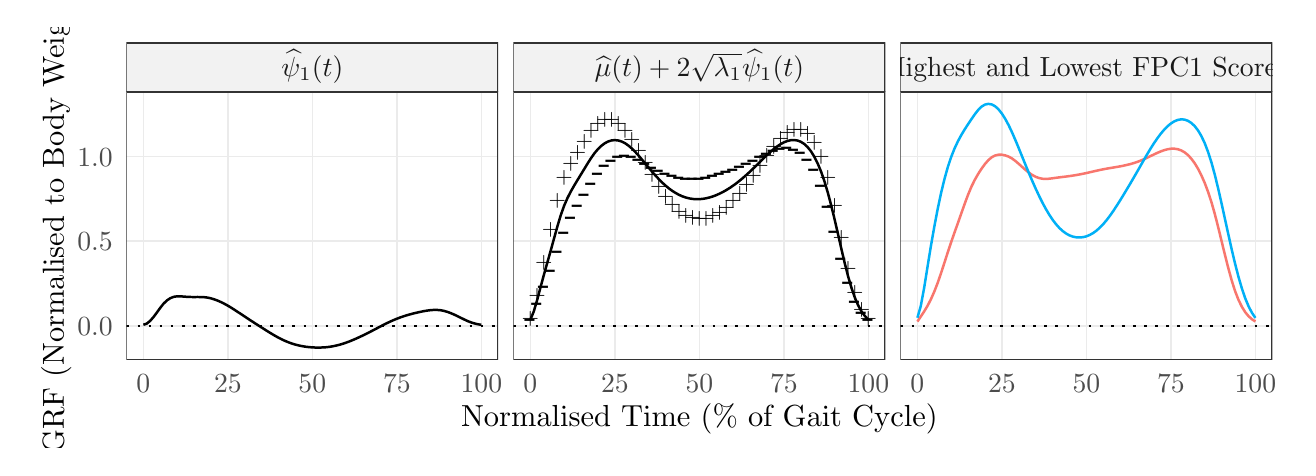
\begin{tikzpicture}[x=1pt,y=1pt]
\definecolor{fillColor}{RGB}{255,255,255}
\path[use as bounding box,fill=fillColor,fill opacity=0.00] (0,0) rectangle (455.24,151.75);
\begin{scope}
\path[clip] (  0.00,  0.00) rectangle (455.24,151.75);
\definecolor{drawColor}{RGB}{255,255,255}
\definecolor{fillColor}{RGB}{255,255,255}

\path[draw=drawColor,line width= 0.6pt,line join=round,line cap=round,fill=fillColor] (  0.00, -0.00) rectangle (455.24,151.75);
\end{scope}
\begin{scope}
\path[clip] ( 35.69, 31.75) rectangle (170.04,128.62);
\definecolor{fillColor}{RGB}{255,255,255}

\path[fill=fillColor] ( 35.69, 31.75) rectangle (170.04,128.62);
\definecolor{drawColor}{gray}{0.92}

\path[draw=drawColor,line width= 0.6pt,line join=round] ( 35.69, 44.04) --
	(170.04, 44.04);

\path[draw=drawColor,line width= 0.6pt,line join=round] ( 35.69, 74.60) --
	(170.04, 74.60);

\path[draw=drawColor,line width= 0.6pt,line join=round] ( 35.69,105.16) --
	(170.04,105.16);

\path[draw=drawColor,line width= 0.6pt,line join=round] ( 41.80, 31.75) --
	( 41.80,128.62);

\path[draw=drawColor,line width= 0.6pt,line join=round] ( 72.33, 31.75) --
	( 72.33,128.62);

\path[draw=drawColor,line width= 0.6pt,line join=round] (102.86, 31.75) --
	(102.86,128.62);

\path[draw=drawColor,line width= 0.6pt,line join=round] (133.40, 31.75) --
	(133.40,128.62);

\path[draw=drawColor,line width= 0.6pt,line join=round] (163.93, 31.75) --
	(163.93,128.62);
\definecolor{drawColor}{RGB}{0,0,0}

\path[draw=drawColor,line width= 0.9pt,line join=round] ( 41.80, 44.39) --
	( 43.02, 44.80) --
	( 44.24, 45.78) --
	( 45.46, 47.17) --
	( 46.68, 48.81) --
	( 47.90, 50.51) --
	( 49.12, 52.04) --
	( 50.35, 53.23) --
	( 51.57, 54.02) --
	( 52.79, 54.49) --
	( 54.01, 54.68) --
	( 55.23, 54.67) --
	( 56.45, 54.57) --
	( 57.67, 54.48) --
	( 58.90, 54.43) --
	( 60.12, 54.42) --
	( 61.34, 54.43) --
	( 62.56, 54.42) --
	( 63.78, 54.36) --
	( 65.00, 54.21) --
	( 66.22, 53.95) --
	( 67.44, 53.57) --
	( 68.67, 53.11) --
	( 69.89, 52.57) --
	( 71.11, 51.96) --
	( 72.33, 51.29) --
	( 73.55, 50.56) --
	( 74.77, 49.78) --
	( 75.99, 48.98) --
	( 77.22, 48.17) --
	( 78.44, 47.36) --
	( 79.66, 46.55) --
	( 80.88, 45.75) --
	( 82.10, 44.96) --
	( 83.32, 44.18) --
	( 84.54, 43.40) --
	( 85.77, 42.62) --
	( 86.99, 41.85) --
	( 88.21, 41.11) --
	( 89.43, 40.39) --
	( 90.65, 39.72) --
	( 91.87, 39.09) --
	( 93.09, 38.53) --
	( 94.32, 38.03) --
	( 95.54, 37.59) --
	( 96.76, 37.22) --
	( 97.98, 36.91) --
	( 99.20, 36.66) --
	(100.42, 36.46) --
	(101.64, 36.32) --
	(102.86, 36.22) --
	(104.09, 36.16) --
	(105.31, 36.15) --
	(106.53, 36.19) --
	(107.75, 36.27) --
	(108.97, 36.41) --
	(110.19, 36.61) --
	(111.41, 36.86) --
	(112.64, 37.16) --
	(113.86, 37.52) --
	(115.08, 37.94) --
	(116.30, 38.39) --
	(117.52, 38.89) --
	(118.74, 39.42) --
	(119.96, 39.98) --
	(121.19, 40.56) --
	(122.41, 41.16) --
	(123.63, 41.78) --
	(124.85, 42.41) --
	(126.07, 43.05) --
	(127.29, 43.69) --
	(128.51, 44.33) --
	(129.73, 44.94) --
	(130.96, 45.52) --
	(132.18, 46.07) --
	(133.40, 46.57) --
	(134.62, 47.04) --
	(135.84, 47.46) --
	(137.06, 47.85) --
	(138.28, 48.19) --
	(139.51, 48.51) --
	(140.73, 48.80) --
	(141.95, 49.07) --
	(143.17, 49.32) --
	(144.39, 49.52) --
	(145.61, 49.68) --
	(146.83, 49.76) --
	(148.06, 49.75) --
	(149.28, 49.63) --
	(150.50, 49.39) --
	(151.72, 49.03) --
	(152.94, 48.58) --
	(154.16, 48.05) --
	(155.38, 47.47) --
	(156.61, 46.86) --
	(157.83, 46.26) --
	(159.05, 45.70) --
	(160.27, 45.23) --
	(161.49, 44.86) --
	(162.71, 44.58) --
	(163.93, 44.37);

\path[draw=drawColor,line width= 0.6pt,dash pattern=on 1pt off 3pt ,line join=round] ( 35.69, 44.04) -- (170.04, 44.04);
\definecolor{drawColor}{gray}{0.20}

\path[draw=drawColor,line width= 0.6pt,line join=round,line cap=round] ( 35.69, 31.75) rectangle (170.04,128.62);
\end{scope}
\begin{scope}
\path[clip] (175.54, 31.75) rectangle (309.89,128.62);
\definecolor{fillColor}{RGB}{255,255,255}

\path[fill=fillColor] (175.54, 31.75) rectangle (309.89,128.62);
\definecolor{drawColor}{gray}{0.92}

\path[draw=drawColor,line width= 0.6pt,line join=round] (175.54, 44.04) --
	(309.89, 44.04);

\path[draw=drawColor,line width= 0.6pt,line join=round] (175.54, 74.60) --
	(309.89, 74.60);

\path[draw=drawColor,line width= 0.6pt,line join=round] (175.54,105.16) --
	(309.89,105.16);

\path[draw=drawColor,line width= 0.6pt,line join=round] (181.65, 31.75) --
	(181.65,128.62);

\path[draw=drawColor,line width= 0.6pt,line join=round] (212.18, 31.75) --
	(212.18,128.62);

\path[draw=drawColor,line width= 0.6pt,line join=round] (242.72, 31.75) --
	(242.72,128.62);

\path[draw=drawColor,line width= 0.6pt,line join=round] (273.25, 31.75) --
	(273.25,128.62);

\path[draw=drawColor,line width= 0.6pt,line join=round] (303.78, 31.75) --
	(303.78,128.62);
\definecolor{drawColor}{RGB}{0,0,0}

\path[draw=drawColor,line width= 0.9pt,line join=round] (181.65, 46.23) --
	(182.87, 49.18) --
	(184.09, 53.31) --
	(185.31, 57.92) --
	(186.53, 62.42) --
	(187.75, 66.78) --
	(188.98, 71.13) --
	(190.20, 75.58) --
	(191.42, 79.97) --
	(192.64, 84.02) --
	(193.86, 87.44) --
	(195.08, 90.25) --
	(196.30, 92.62) --
	(197.53, 94.77) --
	(198.75, 96.81) --
	(199.97, 98.80) --
	(201.19,100.80) --
	(202.41,102.80) --
	(203.63,104.71) --
	(204.85,106.43) --
	(206.07,107.88) --
	(207.30,109.06) --
	(208.52,109.97) --
	(209.74,110.62) --
	(210.96,111.00) --
	(212.18,111.12) --
	(213.40,110.99) --
	(214.62,110.61) --
	(215.85,110.00) --
	(217.07,109.15) --
	(218.29,108.11) --
	(219.51,106.89) --
	(220.73,105.55) --
	(221.95,104.12) --
	(223.17,102.64) --
	(224.40,101.17) --
	(225.62, 99.72) --
	(226.84, 98.33) --
	(228.06, 97.02) --
	(229.28, 95.79) --
	(230.50, 94.67) --
	(231.72, 93.66) --
	(232.95, 92.76) --
	(234.17, 91.99) --
	(235.39, 91.33) --
	(236.61, 90.79) --
	(237.83, 90.37) --
	(239.05, 90.06) --
	(240.27, 89.86) --
	(241.49, 89.77) --
	(242.72, 89.78) --
	(243.94, 89.89) --
	(245.16, 90.10) --
	(246.38, 90.39) --
	(247.60, 90.77) --
	(248.82, 91.24) --
	(250.04, 91.78) --
	(251.27, 92.40) --
	(252.49, 93.09) --
	(253.71, 93.85) --
	(254.93, 94.68) --
	(256.15, 95.58) --
	(257.37, 96.54) --
	(258.59, 97.56) --
	(259.82, 98.64) --
	(261.04, 99.77) --
	(262.26,100.94) --
	(263.48,102.14) --
	(264.70,103.35) --
	(265.92,104.55) --
	(267.14,105.73) --
	(268.36,106.85) --
	(269.59,107.89) --
	(270.81,108.82) --
	(272.03,109.64) --
	(273.25,110.30) --
	(274.47,110.79) --
	(275.69,111.08) --
	(276.91,111.15) --
	(278.14,110.98) --
	(279.36,110.52) --
	(280.58,109.75) --
	(281.80,108.63) --
	(283.02,107.11) --
	(284.24,105.15) --
	(285.46,102.71) --
	(286.69, 99.75) --
	(287.91, 96.23) --
	(289.13, 92.15) --
	(290.35, 87.54) --
	(291.57, 82.53) --
	(292.79, 77.25) --
	(294.01, 71.88) --
	(295.24, 66.67) --
	(296.46, 61.89) --
	(297.68, 57.72) --
	(298.90, 54.21) --
	(300.12, 51.36) --
	(301.34, 49.16) --
	(302.56, 47.50) --
	(303.78, 46.22);

\node[text=drawColor,anchor=base,inner sep=0pt, outer sep=0pt, scale=  0.81] at (181.65, 44.54) {+};

\node[text=drawColor,anchor=base,inner sep=0pt, outer sep=0pt, scale=  0.81] at (184.09, 52.91) {+};

\node[text=drawColor,anchor=base,inner sep=0pt, outer sep=0pt, scale=  0.81] at (186.53, 64.84) {+};

\node[text=drawColor,anchor=base,inner sep=0pt, outer sep=0pt, scale=  0.81] at (188.98, 76.56) {+};

\node[text=drawColor,anchor=base,inner sep=0pt, outer sep=0pt, scale=  0.81] at (191.42, 87.24) {+};

\node[text=drawColor,anchor=base,inner sep=0pt, outer sep=0pt, scale=  0.81] at (193.86, 95.32) {+};

\node[text=drawColor,anchor=base,inner sep=0pt, outer sep=0pt, scale=  0.81] at (196.30,100.40) {+};

\node[text=drawColor,anchor=base,inner sep=0pt, outer sep=0pt, scale=  0.81] at (198.75,104.45) {+};

\node[text=drawColor,anchor=base,inner sep=0pt, outer sep=0pt, scale=  0.81] at (201.19,108.44) {+};

\node[text=drawColor,anchor=base,inner sep=0pt, outer sep=0pt, scale=  0.81] at (203.63,112.29) {+};

\node[text=drawColor,anchor=base,inner sep=0pt, outer sep=0pt, scale=  0.81] at (206.07,115.07) {+};

\node[text=drawColor,anchor=base,inner sep=0pt, outer sep=0pt, scale=  0.81] at (208.52,116.39) {+};

\node[text=drawColor,anchor=base,inner sep=0pt, outer sep=0pt, scale=  0.81] at (210.96,116.35) {+};

\node[text=drawColor,anchor=base,inner sep=0pt, outer sep=0pt, scale=  0.81] at (213.40,115.03) {+};

\node[text=drawColor,anchor=base,inner sep=0pt, outer sep=0pt, scale=  0.81] at (215.85,112.58) {+};

\node[text=drawColor,anchor=base,inner sep=0pt, outer sep=0pt, scale=  0.81] at (218.29,109.18) {+};

\node[text=drawColor,anchor=base,inner sep=0pt, outer sep=0pt, scale=  0.81] at (220.73,105.13) {+};

\node[text=drawColor,anchor=base,inner sep=0pt, outer sep=0pt, scale=  0.81] at (223.17,100.76) {+};

\node[text=drawColor,anchor=base,inner sep=0pt, outer sep=0pt, scale=  0.81] at (225.62, 96.39) {+};

\node[text=drawColor,anchor=base,inner sep=0pt, outer sep=0pt, scale=  0.81] at (228.06, 92.28) {+};

\node[text=drawColor,anchor=base,inner sep=0pt, outer sep=0pt, scale=  0.81] at (230.50, 88.64) {+};

\node[text=drawColor,anchor=base,inner sep=0pt, outer sep=0pt, scale=  0.81] at (232.95, 85.63) {+};

\node[text=drawColor,anchor=base,inner sep=0pt, outer sep=0pt, scale=  0.81] at (235.39, 83.33) {+};

\node[text=drawColor,anchor=base,inner sep=0pt, outer sep=0pt, scale=  0.81] at (237.83, 81.74) {+};

\node[text=drawColor,anchor=base,inner sep=0pt, outer sep=0pt, scale=  0.81] at (240.27, 80.81) {+};

\node[text=drawColor,anchor=base,inner sep=0pt, outer sep=0pt, scale=  0.81] at (242.72, 80.50) {+};

\node[text=drawColor,anchor=base,inner sep=0pt, outer sep=0pt, scale=  0.81] at (245.16, 80.75) {+};

\node[text=drawColor,anchor=base,inner sep=0pt, outer sep=0pt, scale=  0.81] at (247.60, 81.55) {+};

\node[text=drawColor,anchor=base,inner sep=0pt, outer sep=0pt, scale=  0.81] at (250.04, 82.86) {+};

\node[text=drawColor,anchor=base,inner sep=0pt, outer sep=0pt, scale=  0.81] at (252.49, 84.69) {+};

\node[text=drawColor,anchor=base,inner sep=0pt, outer sep=0pt, scale=  0.81] at (254.93, 87.00) {+};

\node[text=drawColor,anchor=base,inner sep=0pt, outer sep=0pt, scale=  0.81] at (257.37, 89.75) {+};

\node[text=drawColor,anchor=base,inner sep=0pt, outer sep=0pt, scale=  0.81] at (259.82, 92.86) {+};

\node[text=drawColor,anchor=base,inner sep=0pt, outer sep=0pt, scale=  0.81] at (262.26, 96.25) {+};

\node[text=drawColor,anchor=base,inner sep=0pt, outer sep=0pt, scale=  0.81] at (264.70, 99.82) {+};

\node[text=drawColor,anchor=base,inner sep=0pt, outer sep=0pt, scale=  0.81] at (267.14,103.39) {+};

\node[text=drawColor,anchor=base,inner sep=0pt, outer sep=0pt, scale=  0.81] at (269.59,106.71) {+};

\node[text=drawColor,anchor=base,inner sep=0pt, outer sep=0pt, scale=  0.81] at (272.03,109.51) {+};

\node[text=drawColor,anchor=base,inner sep=0pt, outer sep=0pt, scale=  0.81] at (274.47,111.56) {+};

\node[text=drawColor,anchor=base,inner sep=0pt, outer sep=0pt, scale=  0.81] at (276.91,112.68) {+};

\node[text=drawColor,anchor=base,inner sep=0pt, outer sep=0pt, scale=  0.81] at (279.36,112.66) {+};

\node[text=drawColor,anchor=base,inner sep=0pt, outer sep=0pt, scale=  0.81] at (281.80,111.29) {+};

\node[text=drawColor,anchor=base,inner sep=0pt, outer sep=0pt, scale=  0.81] at (284.24,108.24) {+};

\node[text=drawColor,anchor=base,inner sep=0pt, outer sep=0pt, scale=  0.81] at (286.69,103.05) {+};

\node[text=drawColor,anchor=base,inner sep=0pt, outer sep=0pt, scale=  0.81] at (289.13, 95.33) {+};

\node[text=drawColor,anchor=base,inner sep=0pt, outer sep=0pt, scale=  0.81] at (291.57, 85.16) {+};

\node[text=drawColor,anchor=base,inner sep=0pt, outer sep=0pt, scale=  0.81] at (294.01, 73.59) {+};

\node[text=drawColor,anchor=base,inner sep=0pt, outer sep=0pt, scale=  0.81] at (296.46, 62.50) {+};

\node[text=drawColor,anchor=base,inner sep=0pt, outer sep=0pt, scale=  0.81] at (298.90, 53.74) {+};

\node[text=drawColor,anchor=base,inner sep=0pt, outer sep=0pt, scale=  0.81] at (301.34, 47.92) {+};

\node[text=drawColor,anchor=base,inner sep=0pt, outer sep=0pt, scale=  0.81] at (303.78, 44.51) {+};

\node[text=drawColor,anchor=base,inner sep=0pt, outer sep=0pt, scale=  1.37] at (181.65, 42.94) {-};

\node[text=drawColor,anchor=base,inner sep=0pt, outer sep=0pt, scale=  1.37] at (184.09, 48.73) {-};

\node[text=drawColor,anchor=base,inner sep=0pt, outer sep=0pt, scale=  1.37] at (186.53, 55.03) {-};

\node[text=drawColor,anchor=base,inner sep=0pt, outer sep=0pt, scale=  1.37] at (188.98, 60.73) {-};

\node[text=drawColor,anchor=base,inner sep=0pt, outer sep=0pt, scale=  1.37] at (191.42, 67.73) {-};

\node[text=drawColor,anchor=base,inner sep=0pt, outer sep=0pt, scale=  1.37] at (193.86, 74.59) {-};

\node[text=drawColor,anchor=base,inner sep=0pt, outer sep=0pt, scale=  1.37] at (196.30, 79.87) {-};

\node[text=drawColor,anchor=base,inner sep=0pt, outer sep=0pt, scale=  1.37] at (198.75, 84.19) {-};

\node[text=drawColor,anchor=base,inner sep=0pt, outer sep=0pt, scale=  1.37] at (201.19, 88.18) {-};

\node[text=drawColor,anchor=base,inner sep=0pt, outer sep=0pt, scale=  1.37] at (203.63, 92.16) {-};

\node[text=drawColor,anchor=base,inner sep=0pt, outer sep=0pt, scale=  1.37] at (206.07, 95.71) {-};

\node[text=drawColor,anchor=base,inner sep=0pt, outer sep=0pt, scale=  1.37] at (208.52, 98.58) {-};

\node[text=drawColor,anchor=base,inner sep=0pt, outer sep=0pt, scale=  1.37] at (210.96,100.67) {-};

\node[text=drawColor,anchor=base,inner sep=0pt, outer sep=0pt, scale=  1.37] at (213.40,101.97) {-};

\node[text=drawColor,anchor=base,inner sep=0pt, outer sep=0pt, scale=  1.37] at (215.85,102.44) {-};

\node[text=drawColor,anchor=base,inner sep=0pt, outer sep=0pt, scale=  1.37] at (218.29,102.06) {-};

\node[text=drawColor,anchor=base,inner sep=0pt, outer sep=0pt, scale=  1.37] at (220.73,101.00) {-};

\node[text=drawColor,anchor=base,inner sep=0pt, outer sep=0pt, scale=  1.37] at (223.17, 99.55) {-};

\node[text=drawColor,anchor=base,inner sep=0pt, outer sep=0pt, scale=  1.37] at (225.62, 98.08) {-};

\node[text=drawColor,anchor=base,inner sep=0pt, outer sep=0pt, scale=  1.37] at (228.06, 96.78) {-};

\node[text=drawColor,anchor=base,inner sep=0pt, outer sep=0pt, scale=  1.37] at (230.50, 95.73) {-};

\node[text=drawColor,anchor=base,inner sep=0pt, outer sep=0pt, scale=  1.37] at (232.95, 94.92) {-};

\node[text=drawColor,anchor=base,inner sep=0pt, outer sep=0pt, scale=  1.37] at (235.39, 94.36) {-};

\node[text=drawColor,anchor=base,inner sep=0pt, outer sep=0pt, scale=  1.37] at (237.83, 94.03) {-};

\node[text=drawColor,anchor=base,inner sep=0pt, outer sep=0pt, scale=  1.37] at (240.27, 93.94) {-};

\node[text=drawColor,anchor=base,inner sep=0pt, outer sep=0pt, scale=  1.37] at (242.72, 94.09) {-};

\node[text=drawColor,anchor=base,inner sep=0pt, outer sep=0pt, scale=  1.37] at (245.16, 94.46) {-};

\node[text=drawColor,anchor=base,inner sep=0pt, outer sep=0pt, scale=  1.37] at (247.60, 95.03) {-};

\node[text=drawColor,anchor=base,inner sep=0pt, outer sep=0pt, scale=  1.37] at (250.04, 95.72) {-};

\node[text=drawColor,anchor=base,inner sep=0pt, outer sep=0pt, scale=  1.37] at (252.49, 96.52) {-};

\node[text=drawColor,anchor=base,inner sep=0pt, outer sep=0pt, scale=  1.37] at (254.93, 97.39) {-};

\node[text=drawColor,anchor=base,inner sep=0pt, outer sep=0pt, scale=  1.37] at (257.37, 98.36) {-};

\node[text=drawColor,anchor=base,inner sep=0pt, outer sep=0pt, scale=  1.37] at (259.82, 99.45) {-};

\node[text=drawColor,anchor=base,inner sep=0pt, outer sep=0pt, scale=  1.37] at (262.26,100.66) {-};

\node[text=drawColor,anchor=base,inner sep=0pt, outer sep=0pt, scale=  1.37] at (264.70,101.90) {-};

\node[text=drawColor,anchor=base,inner sep=0pt, outer sep=0pt, scale=  1.37] at (267.14,103.09) {-};

\node[text=drawColor,anchor=base,inner sep=0pt, outer sep=0pt, scale=  1.37] at (269.59,104.09) {-};

\node[text=drawColor,anchor=base,inner sep=0pt, outer sep=0pt, scale=  1.37] at (272.03,104.79) {-};

\node[text=drawColor,anchor=base,inner sep=0pt, outer sep=0pt, scale=  1.37] at (274.47,105.04) {-};

\node[text=drawColor,anchor=base,inner sep=0pt, outer sep=0pt, scale=  1.37] at (276.91,104.65) {-};

\node[text=drawColor,anchor=base,inner sep=0pt, outer sep=0pt, scale=  1.37] at (279.36,103.40) {-};

\node[text=drawColor,anchor=base,inner sep=0pt, outer sep=0pt, scale=  1.37] at (281.80,100.99) {-};

\node[text=drawColor,anchor=base,inner sep=0pt, outer sep=0pt, scale=  1.37] at (284.24, 97.10) {-};

\node[text=drawColor,anchor=base,inner sep=0pt, outer sep=0pt, scale=  1.37] at (286.69, 91.47) {-};

\node[text=drawColor,anchor=base,inner sep=0pt, outer sep=0pt, scale=  1.37] at (289.13, 83.99) {-};

\node[text=drawColor,anchor=base,inner sep=0pt, outer sep=0pt, scale=  1.37] at (291.57, 74.93) {-};

\node[text=drawColor,anchor=base,inner sep=0pt, outer sep=0pt, scale=  1.37] at (294.01, 65.19) {-};

\node[text=drawColor,anchor=base,inner sep=0pt, outer sep=0pt, scale=  1.37] at (296.46, 56.31) {-};

\node[text=drawColor,anchor=base,inner sep=0pt, outer sep=0pt, scale=  1.37] at (298.90, 49.70) {-};

\node[text=drawColor,anchor=base,inner sep=0pt, outer sep=0pt, scale=  1.37] at (301.34, 45.44) {-};

\node[text=drawColor,anchor=base,inner sep=0pt, outer sep=0pt, scale=  1.37] at (303.78, 42.95) {-};

\path[draw=drawColor,line width= 0.6pt,dash pattern=on 1pt off 3pt ,line join=round] (175.54, 44.04) -- (309.89, 44.04);
\definecolor{drawColor}{gray}{0.20}

\path[draw=drawColor,line width= 0.6pt,line join=round,line cap=round] (175.54, 31.75) rectangle (309.89,128.62);
\end{scope}
\begin{scope}
\path[clip] (315.39, 31.75) rectangle (449.74,128.62);
\definecolor{fillColor}{RGB}{255,255,255}

\path[fill=fillColor] (315.39, 31.75) rectangle (449.74,128.62);
\definecolor{drawColor}{gray}{0.92}

\path[draw=drawColor,line width= 0.6pt,line join=round] (315.39, 44.04) --
	(449.74, 44.04);

\path[draw=drawColor,line width= 0.6pt,line join=round] (315.39, 74.60) --
	(449.74, 74.60);

\path[draw=drawColor,line width= 0.6pt,line join=round] (315.39,105.16) --
	(449.74,105.16);

\path[draw=drawColor,line width= 0.6pt,line join=round] (321.50, 31.75) --
	(321.50,128.62);

\path[draw=drawColor,line width= 0.6pt,line join=round] (352.03, 31.75) --
	(352.03,128.62);

\path[draw=drawColor,line width= 0.6pt,line join=round] (382.57, 31.75) --
	(382.57,128.62);

\path[draw=drawColor,line width= 0.6pt,line join=round] (413.10, 31.75) --
	(413.10,128.62);

\path[draw=drawColor,line width= 0.6pt,line join=round] (443.64, 31.75) --
	(443.64,128.62);
\definecolor{drawColor}{RGB}{248,118,109}

\path[draw=drawColor,line width= 0.9pt,line join=round] (321.50, 45.54) --
	(322.72, 47.37) --
	(323.94, 49.20) --
	(325.16, 51.23) --
	(326.38, 53.61) --
	(327.61, 56.38) --
	(328.83, 59.54) --
	(330.05, 63.07) --
	(331.27, 66.83) --
	(332.49, 70.64) --
	(333.71, 74.29) --
	(334.93, 77.79) --
	(336.16, 81.22) --
	(337.38, 84.69) --
	(338.60, 88.14) --
	(339.82, 91.42) --
	(341.04, 94.33) --
	(342.26, 96.81) --
	(343.48, 98.94) --
	(344.70,100.83) --
	(345.93,102.50) --
	(347.15,103.90) --
	(348.37,104.93) --
	(349.59,105.56) --
	(350.81,105.84) --
	(352.03,105.84) --
	(353.25,105.60) --
	(354.48,105.15) --
	(355.70,104.47) --
	(356.92,103.57) --
	(358.14,102.53) --
	(359.36,101.42) --
	(360.58,100.34) --
	(361.80, 99.35) --
	(363.03, 98.51) --
	(364.25, 97.85) --
	(365.47, 97.41) --
	(366.69, 97.16) --
	(367.91, 97.09) --
	(369.13, 97.17) --
	(370.35, 97.33) --
	(371.58, 97.50) --
	(372.80, 97.66) --
	(374.02, 97.81) --
	(375.24, 97.96) --
	(376.46, 98.12) --
	(377.68, 98.30) --
	(378.90, 98.50) --
	(380.12, 98.72) --
	(381.35, 98.96) --
	(382.57, 99.22) --
	(383.79, 99.50) --
	(385.01, 99.78) --
	(386.23,100.06) --
	(387.45,100.33) --
	(388.67,100.58) --
	(389.90,100.81) --
	(391.12,101.02) --
	(392.34,101.22) --
	(393.56,101.43) --
	(394.78,101.64) --
	(396.00,101.88) --
	(397.22,102.16) --
	(398.45,102.46) --
	(399.67,102.82) --
	(400.89,103.22) --
	(402.11,103.69) --
	(403.33,104.21) --
	(404.55,104.77) --
	(405.77,105.36) --
	(407.00,105.95) --
	(408.22,106.52) --
	(409.44,107.04) --
	(410.66,107.48) --
	(411.88,107.81) --
	(413.10,108.00) --
	(414.32,108.02) --
	(415.54,107.84) --
	(416.77,107.42) --
	(417.99,106.74) --
	(419.21,105.76) --
	(420.43,104.47) --
	(421.65,102.83) --
	(422.87,100.83) --
	(424.09, 98.44) --
	(425.32, 95.65) --
	(426.54, 92.41) --
	(427.76, 88.67) --
	(428.98, 84.37) --
	(430.20, 79.61) --
	(431.42, 74.60) --
	(432.64, 69.59) --
	(433.87, 64.77) --
	(435.09, 60.35) --
	(436.31, 56.52) --
	(437.53, 53.38) --
	(438.75, 50.88) --
	(439.97, 48.93) --
	(441.19, 47.46) --
	(442.41, 46.37) --
	(443.64, 45.58);
\definecolor{drawColor}{RGB}{0,176,246}

\path[draw=drawColor,line width= 0.9pt,line join=round] (321.50, 46.94) --
	(322.72, 51.17) --
	(323.94, 57.74) --
	(325.16, 65.36) --
	(326.38, 72.85) --
	(327.61, 79.84) --
	(328.83, 86.24) --
	(330.05, 91.98) --
	(331.27, 97.02) --
	(332.49,101.37) --
	(333.71,105.04) --
	(334.93,108.12) --
	(336.16,110.73) --
	(337.38,112.99) --
	(338.60,115.01) --
	(339.82,116.89) --
	(341.04,118.71) --
	(342.26,120.47) --
	(343.48,122.03) --
	(344.70,123.23) --
	(345.93,123.96) --
	(347.15,124.21) --
	(348.37,124.01) --
	(349.59,123.35) --
	(350.81,122.24) --
	(352.03,120.71) --
	(353.25,118.77) --
	(354.48,116.49) --
	(355.70,113.91) --
	(356.92,111.11) --
	(358.14,108.16) --
	(359.36,105.14) --
	(360.58,102.14) --
	(361.80, 99.18) --
	(363.03, 96.31) --
	(364.25, 93.56) --
	(365.47, 90.96) --
	(366.69, 88.51) --
	(367.91, 86.25) --
	(369.13, 84.19) --
	(370.35, 82.34) --
	(371.58, 80.74) --
	(372.80, 79.37) --
	(374.02, 78.25) --
	(375.24, 77.36) --
	(376.46, 76.69) --
	(377.68, 76.24) --
	(378.90, 75.99) --
	(380.12, 75.93) --
	(381.35, 76.05) --
	(382.57, 76.36) --
	(383.79, 76.86) --
	(385.01, 77.55) --
	(386.23, 78.43) --
	(387.45, 79.52) --
	(388.67, 80.79) --
	(389.90, 82.24) --
	(391.12, 83.85) --
	(392.34, 85.60) --
	(393.56, 87.46) --
	(394.78, 89.39) --
	(396.00, 91.37) --
	(397.22, 93.40) --
	(398.45, 95.47) --
	(399.67, 97.56) --
	(400.89, 99.68) --
	(402.11,101.82) --
	(403.33,103.96) --
	(404.55,106.06) --
	(405.77,108.09) --
	(407.00,110.01) --
	(408.22,111.80) --
	(409.44,113.43) --
	(410.66,114.87) --
	(411.88,116.11) --
	(413.10,117.13) --
	(414.32,117.90) --
	(415.54,118.40) --
	(416.77,118.62) --
	(417.99,118.54) --
	(419.21,118.12) --
	(420.43,117.36) --
	(421.65,116.23) --
	(422.87,114.67) --
	(424.09,112.62) --
	(425.32,110.02) --
	(426.54,106.82) --
	(427.76,103.01) --
	(428.98, 98.56) --
	(430.20, 93.56) --
	(431.42, 88.17) --
	(432.64, 82.59) --
	(433.87, 76.99) --
	(435.09, 71.53) --
	(436.31, 66.38) --
	(437.53, 61.68) --
	(438.75, 57.51) --
	(439.97, 53.94) --
	(441.19, 51.01) --
	(442.41, 48.68) --
	(443.64, 46.88);
\definecolor{drawColor}{RGB}{0,0,0}

\path[draw=drawColor,line width= 0.6pt,dash pattern=on 1pt off 3pt ,line join=round] (315.39, 44.04) -- (449.74, 44.04);
\definecolor{drawColor}{gray}{0.20}

\path[draw=drawColor,line width= 0.6pt,line join=round,line cap=round] (315.39, 31.75) rectangle (449.74,128.62);
\end{scope}
\begin{scope}
\path[clip] ( 35.69,128.62) rectangle (170.04,146.25);
\definecolor{drawColor}{gray}{0.20}
\definecolor{fillColor}{RGB}{190,190,190}

\path[draw=drawColor,line width= 0.6pt,line join=round,line cap=round,fill=fillColor,fill opacity=0.20] ( 35.69,128.62) rectangle (170.04,146.25);
\definecolor{drawColor}{gray}{0.10}

\node[text=drawColor,anchor=base,inner sep=0pt, outer sep=0pt, scale=  1.00] at (102.86,133.99) {$\widehat{\psi}_1 (t)$};
\end{scope}
\begin{scope}
\path[clip] (175.54,128.62) rectangle (309.89,146.25);
\definecolor{drawColor}{gray}{0.20}
\definecolor{fillColor}{RGB}{190,190,190}

\path[draw=drawColor,line width= 0.6pt,line join=round,line cap=round,fill=fillColor,fill opacity=0.20] (175.54,128.62) rectangle (309.89,146.25);
\definecolor{drawColor}{gray}{0.10}

\node[text=drawColor,anchor=base,inner sep=0pt, outer sep=0pt, scale=  1.00] at (242.72,133.99) {$\widehat{\mu} (t) + 2 \sqrt{\lambda_1} \widehat{\psi}_1 (t)$};
\end{scope}
\begin{scope}
\path[clip] (315.39,128.62) rectangle (449.74,146.25);
\definecolor{drawColor}{gray}{0.20}
\definecolor{fillColor}{RGB}{190,190,190}

\path[draw=drawColor,line width= 0.6pt,line join=round,line cap=round,fill=fillColor,fill opacity=0.20] (315.39,128.62) rectangle (449.74,146.25);
\definecolor{drawColor}{gray}{0.10}

\node[text=drawColor,anchor=base,inner sep=0pt, outer sep=0pt, scale=  1.00] at (382.57,133.99) {Highest and Lowest FPC1 Scores};
\end{scope}
\begin{scope}
\path[clip] (  0.00,  0.00) rectangle (455.24,151.75);
\definecolor{drawColor}{gray}{0.30}

\node[text=drawColor,anchor=base,inner sep=0pt, outer sep=0pt, scale=  1.00] at ( 41.80, 19.91) {0};

\node[text=drawColor,anchor=base,inner sep=0pt, outer sep=0pt, scale=  1.00] at ( 72.33, 19.91) {25};

\node[text=drawColor,anchor=base,inner sep=0pt, outer sep=0pt, scale=  1.00] at (102.86, 19.91) {50};

\node[text=drawColor,anchor=base,inner sep=0pt, outer sep=0pt, scale=  1.00] at (133.40, 19.91) {75};

\node[text=drawColor,anchor=base,inner sep=0pt, outer sep=0pt, scale=  1.00] at (163.93, 19.91) {100};
\end{scope}
\begin{scope}
\path[clip] (  0.00,  0.00) rectangle (455.24,151.75);
\definecolor{drawColor}{gray}{0.30}

\node[text=drawColor,anchor=base,inner sep=0pt, outer sep=0pt, scale=  1.00] at (181.65, 19.91) {0};

\node[text=drawColor,anchor=base,inner sep=0pt, outer sep=0pt, scale=  1.00] at (212.18, 19.91) {25};

\node[text=drawColor,anchor=base,inner sep=0pt, outer sep=0pt, scale=  1.00] at (242.72, 19.91) {50};

\node[text=drawColor,anchor=base,inner sep=0pt, outer sep=0pt, scale=  1.00] at (273.25, 19.91) {75};

\node[text=drawColor,anchor=base,inner sep=0pt, outer sep=0pt, scale=  1.00] at (303.78, 19.91) {100};
\end{scope}
\begin{scope}
\path[clip] (  0.00,  0.00) rectangle (455.24,151.75);
\definecolor{drawColor}{gray}{0.30}

\node[text=drawColor,anchor=base,inner sep=0pt, outer sep=0pt, scale=  1.00] at (321.50, 19.91) {0};

\node[text=drawColor,anchor=base,inner sep=0pt, outer sep=0pt, scale=  1.00] at (352.03, 19.91) {25};

\node[text=drawColor,anchor=base,inner sep=0pt, outer sep=0pt, scale=  1.00] at (382.57, 19.91) {50};

\node[text=drawColor,anchor=base,inner sep=0pt, outer sep=0pt, scale=  1.00] at (413.10, 19.91) {75};

\node[text=drawColor,anchor=base,inner sep=0pt, outer sep=0pt, scale=  1.00] at (443.64, 19.91) {100};
\end{scope}
\begin{scope}
\path[clip] (  0.00,  0.00) rectangle (455.24,151.75);
\definecolor{drawColor}{gray}{0.30}

\node[text=drawColor,anchor=base east,inner sep=0pt, outer sep=0pt, scale=  1.00] at ( 30.74, 40.59) {0.0};

\node[text=drawColor,anchor=base east,inner sep=0pt, outer sep=0pt, scale=  1.00] at ( 30.74, 71.16) {0.5};

\node[text=drawColor,anchor=base east,inner sep=0pt, outer sep=0pt, scale=  1.00] at ( 30.74,101.72) {1.0};
\end{scope}
\begin{scope}
\path[clip] (  0.00,  0.00) rectangle (455.24,151.75);
\definecolor{drawColor}{RGB}{0,0,0}

\node[text=drawColor,anchor=base,inner sep=0pt, outer sep=0pt, scale=  1.10] at (242.72,  7.64) {Normalised Time ($\%$ of Gait Cycle)};
\end{scope}
\begin{scope}
\path[clip] (  0.00,  0.00) rectangle (455.24,151.75);
\definecolor{drawColor}{RGB}{0,0,0}

\node[text=drawColor,rotate= 90.00,anchor=base,inner sep=0pt, outer sep=0pt, scale=  1.10] at ( 13.08, 80.18) {vGRF (Normalised to Body Weight)};
\end{scope}
\end{tikzpicture}
